\documentclass[12pt,fleqn]{article}\usepackage{../../common}
\begin{document}
Calculus'un Temel Teoremi (The Fundamental Theorem of Calculus)

Ana teoriyi ispatlamadan önce iki diğer teoriden bahsetmemiz, ispatlamamız
lazım. Bu teorilerden biri Geçiş Değeri Teorisi (Intermediate Value
Theorem) diğeri Belirli Entegraller İçin Ortalama Değer Teoremi (Mean Value
Theorem for Definite Integrals). Geçiş Değeri Teorisi basitçe şunu söyler

Teori

$[a,b]$ aralığında sürekli bir fonksiyon $y=f(x)$, $f(a)$ ve $f(b)$
arasındaki her değeri muhakkak alır. Bir diğer değişle, eğer $y_o$, $f(a)$
ve $f(b)$ arasındaki bir değer ise $[a,b]$ aralığındaki bir $c$ için
muhakkak $y_0 = f(c)$ olmalıdır. 

Geometrik olarak bu teori $y$ eksenini $f(a)$ ve $f(b)$ arasında kesen
$y=y_0$ yatay çizgisinin $y=f(x)$ fonksiyonunu muhakkak, en az bir kez
keseceğidir. Grafik altta. 

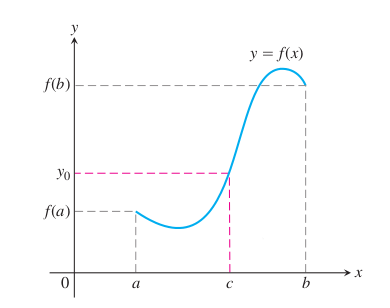
\includegraphics[height=4cm]{calc_multi_app_05.png}

Sezgisel olarak bu anlamlı değil mi? Eğer sürekli bir fonksiyon var ise,
$f(a)$'dan $f(b)$'ye giderken o aralıktaki her sayıya bir kez ``uğramaya''
mecburuz. Etraflarından dolaşmamız mümkün değil, çünkü kesintili bir
fonksiyon değil, kesintisiz / sürekli bir fonksiyonumuz var. Bu teorinin
daha detaylı ispatı için [1]'e bakılabilir. 

Maks-Min Eşitsizliği

Eğer $[a,b]$ aralığında $f$, maksimum değer $\max f$'e ve minimum değer
$min \ f$'e sahipse, 

$$ \min f \cdot (b-a) \le \int_a^b f(x) \ud x \le \max f \cdot (b-a) $$

demektir. 

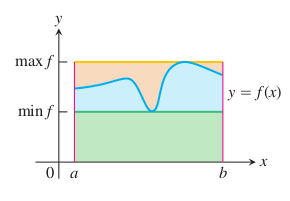
\includegraphics[height=4cm]{calc_multi_app_08.png}

Bu kural diyor ki $f$'in $[a,b]$ üzerindeki entegrali hiçbir zaman $f$'in
minimum'u çarpı $[a,b]$ aralığının uzunluğu'ndan küçük olamaz, ve $f$'in
maksimumu çarpı $[a,b]$ aralığının uzunluğu'ndan büyük olamaz. 

İspat

Eğer $(b-a)$'yi $ \sum_{k=1}^n \Delta x_k$ olarak görürsek

$$ \min \ f \cdot (b-a) = \min \ f \cdot \sum_{k=1}^n \Delta x_k $$
$$  = \sum_{k=1}^n \min \ f \cdot \Delta x_k  $$

$[a,b]$ aralığındaki herhangi bir değer $c_k$ için

$$  \le \sum_{k=1}^n f(c_k) \cdot \Delta x_k  $$

Öyle değil mi? $min \ f$ değeri en küçük değer ise, $[a,b]$ aralığındaki
herhangi bir nokta $c_k$'nin $f$ değeri bu değere ya eşit, ya da ondan
büyüktür. Yani $min \ f \le f(c_k)$. Devam edersek

$$  \le \sum_{k=1}^n \max f \cdot \Delta x_k  $$

Üstteki benzer mantığı takip ediyor, bu sefer $f(c_k) \le \max f $. Son
ifadedeki $max$'i dışarı alabiliriz. 

$$ = \max f \sum_{k=1}^n \cdot \Delta x_k  $$

$$ = \max f (b-a)  $$

Rolle'nin Teorisi

Bir sonraki teoriyi ispatlamadan önce orada gerekli Rolle'nin Teorisinden
bahsetmek lazım. Bu teoriyi ispatlamadan vereceğiz, kabaca doğru olduğunu
anlayabiliriz, teori der ki, eğer bir fonksiyon $f$ 1) $[a,b]$ kapalı bölgesinde
sürekli 2) (a,b) açık aralığında türevi alınabilir ve $f(a)=f(b)$ ise o zaman
bir aynı aralıkta $f'(c)=0$ olacak şekilde bir $c$ varlığı kesindir.

Altta bazı örnekler görüyoruz,

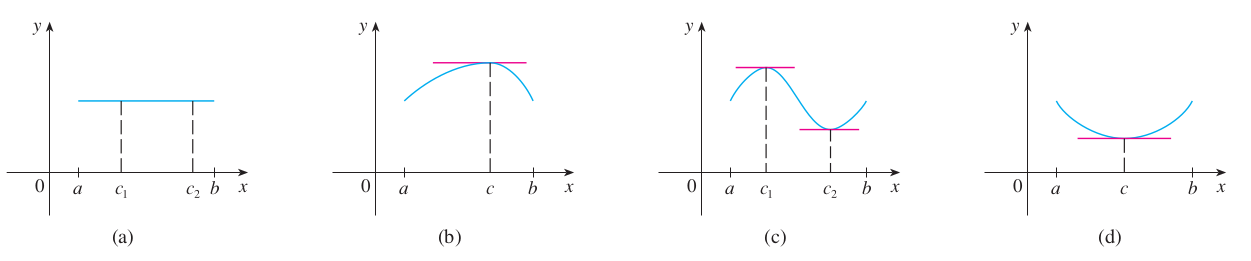
\includegraphics[width=30em]{calc_multi_app_02.png}

Tarif etmek gerekirse iki nokta arasında başı ve sonu aynı olan bir fonksiyon o
arada bir noktada muhakkak tepe, ya da dip noktasına varmış olmalıdır, yani
türevi orada sıfır olmalıdır. Bu sezgisel olarak akla yatkın bir önerme
herhalde. İspat için [2, sf. 281].

Ortalama Değer Teoremi (Türevli Form)

Eğer $f$ fonksiyonu açık aralığında (interval) $(a,b)$ türevi alınabilir halde
ise ve kapalı aralıkta $[a,b]$ sürekli ise, o zaman $(a,b)$ aralığında
en az bir $c$ değeri vardır ki bu değer için

$$
f'(c) = \frac{f(b) - f(a)}{b-a}
$$

doğrudur.

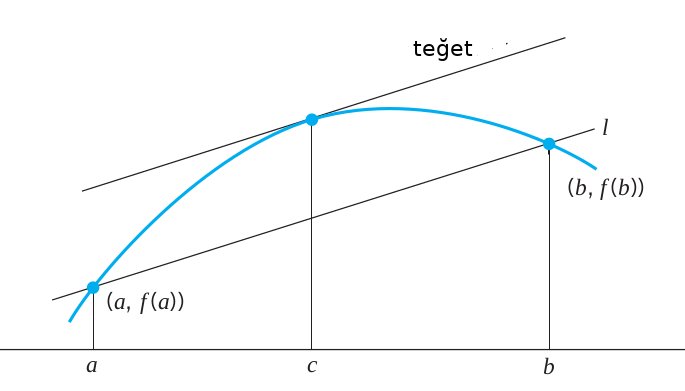
\includegraphics[width=20em]{calc_multi_app_01.png}

Bu teorinin de ispatı için [2, sf. 282]'ye bakılabilir, fakat yine kabaca takip
edilen tekniği tarif edeilm; eğer üstteki grafiği sağa doğru yatırırsak, yani o
$l$ çizgisi tam $x$ eksenine paralel olacak şekilde saat yönüne doğru her şeyi
çevirirsek, yeni $f(a)$ ve $f(b)$ aynı $y$ seviyesinde olacaklar, eh bu durumda
Rolle Teorisi kullanılabilir, ve oradan gelen $c$ olma mecburiyetini ilk
grafiğe tercüme edersek oradaki $c$ varlığını da ispatlamış oluruz. 

Ortalama Değer Teoremi (Entegral Form)

Eğer $f$ fonksiyonu $[a,b]$ arasında sürekli ise o zaman $[a,b]$ aralığında
olan bir $c$ noktasında

$$ f(c) = \frac{1}{b-a}\int_a^b f(x) \ud x $$

eşitliği doğru olmalıdır. Yani alttaki resimde sol grafikteki mavi alanın
$b-a$ ile bölünerek elde edilen ortalama değeri, $[a,b]$ aralığındaki bir
$c$ üzerinden $f(c)$'ye muhakkak eşittir. Ya da bir kenarı $f(c)$, diğeri
$b-a$ olan bir diktortgenin alanı (alt sağdaki resim), mavi alanın
tamamına eşit olacaktır.

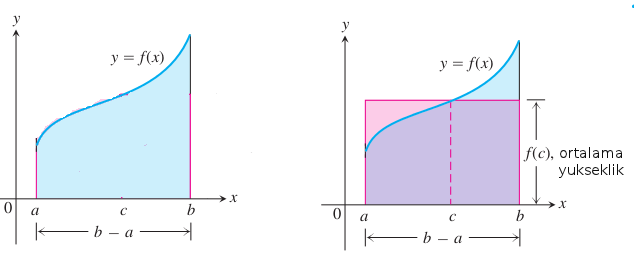
\includegraphics[height=4cm]{calc_multi_app_07.png}

Maks-Min Eşitsizliğinin iki tarafını $b-a$'ya bölersek

$$ \min f  \le \frac{1}{b-a} \int_a^b f(x) \ud x \le \max f  $$

elde ederiz. Eğer Geçiş Değeri Teorisi doğruysa, $\min f$ ve $\max f$
arasındaki tüm noktalar ziyaret edilmelidir. O zaman böyle bir $f(c)$
kesinlikle var demektir.

Calculus'un Temel Teoremi

Teori

Eğer $f$ fonksiyonu $[a,b]$ arasında sürekli ise o zaman 

$$ F(x) = \int_a^x f(t) \ud t  $$

fonksiyonu da $[a,b]$ arasında süreklidir, ve bu fonksiyonun türevi
$f(x)$'in kendisidir.

Yani

$$ F'(x) = \frac{d}{dx}\int_a^x f(t) \ud t = f(x)   $$

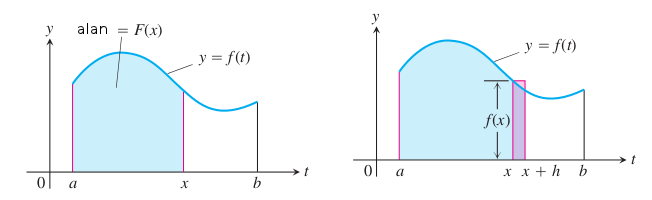
\includegraphics[height=3cm]{calc_multi_app_03.png}

İspat

Türevin tanımını direk $F(x)$ üzerinde uygulayalım, $[a,b]$ içinde olan $x$
ve $x+h$ aralığını alalım, ve

$$ \frac{F(x+h)-F(x)}{h} $$

bölümünün limitinin, $h \to 0$ iken, $f(x)$'e gittiğini göstermeye
çalışalım. $F(x+h)$ ve $F(x)$ fonksiyonlarını entegralleri üzerinden
tanımlayalım. O zaman üstteki formülün bölüm kısmı

$$ F(x+h) - F(x) = \int_a^{x+h} f(t) \ud t - \int_a^x f(t) \ud t  $$

Entegrallerin toplam kuralına göre üstteki formülün sağ tarafı 

$$ \int_x^{x+h} f(t) \ud t  $$

ifadesidir. O zaman bölümün tamamı

$$ \frac{F(x+h)-F(x)}{h} = \frac{1}{h} \int_x^{x+h} f(t) \ud t   $$

Ortalama Değer Teoremine göre, üstteki eşitliğin sağındaki ifadenin, $x$ ve
$x+h$ aralığında $f$'in aldığı değerlerden birine aynen eşit olduğunu
biliyoruz. Yani o aralıktaki bir $c$ için

$$ \frac{1}{h} \int_x^{x+h} f(t) \ud t = f(c) $$

kesinlikle doğru olmalı. Şimdi, $h \to 0$ oldukça, $x+h$ mecburen $x$'e
yaklaşmak zorunda kalacaktır, çünkü $c$, $x$ ile $x+h$ arasında sıkışıp
kalmıştır. $f$ fonksiyonu $x$ noktasında sürekli olduğuna göre, o zaman
$f(c)$, $f(x)$'e yaklaşmalıdır. 

$$ \lim_{h \to 0} f(c) = f(x) $$

Şimdi elimizdeki bu bilgiyle başa dönersek, 

$$ \frac{dF}{dx} = \lim_{h \to 0} \frac{F(x+h)-F(x)}{h} $$

$$  = \lim_{h \to 0} \frac{1}{h} \int_x^{x+h} f(t) \ud t   $$

$$ = \lim_{h \to 0} f(c) $$

$$ = f(x) $$

Ek olarak ilgili bir teori daha gösterelim.

Cauchy Ortalama Değer Teorisi (Cauchy Mean-value Theorem)

Teori şöyle

Eğer $f,g$ fonksiyonları $[a,b]$ aralığında sürekli ise ve $g'(x) \ne 0$
farz edildiği durumda $[a,b]$ arasında öyle bir $c$ vardır ki,

$$ \frac{f'(c)}{g'(c)} = \frac{f(b)-f(a)}{g(b)-g(a)} $$

ifadesi doğrudur. 

İspat

Şimdi daha önceden gördüğümüz Ortalama Değer Teorisi'ni (Cauchy olmayan)
iki kere kullanacağız. Teoriyi önce $g(a) \ne g(b)$ olduğunu göstermek için
kullanacağız. Çünkü eğer bu doğru olsaydı, Ortalama Değer Teorisi 

$$ g'(c) = \frac{g(b) - g(a)}{b-a} = 0$$

olurdu, ki bu $[a,b]$ arasındaki bir $c$ için başta yaptığımız faraziyemiz
$g'(x) \ne 0$ ile ters düşerdi. 

İkinci kullanım: $F(x)$ adında, $f,g$ fonksiyonlarını kullanan başka bir
fonksiyon kurgulayalım.

$$ F(x) = f(x) - f(a) - \frac{f(b)-f(a) }{g(b)-g(a)}[g(x)-g(a)] $$

Bu fonksiyonun türevi, $f,g$'nin türevi alınabildiği her yerde alınabilir
olur. Ayrıca $F(b) = F(a) = 0$. $a,b$ değerlerini yerine koyarsak bunu
görebiliriz, mesela $x=a$ için

$$ F(a) = \cancelto{0}{f(a) - f(a)} -
\frac{f(b)-f(a) }{g(b)-g(a)}
[\cancelto{0}{g(a)-g(a)}] 
$$

$$  = 0 - 0 = 0 $$

O zaman, $F(b) = F(a) = 0$'dan bir sonuca daha erişiriz. Bir fonksiyon
$a,b$ uçlarında sıfır ise, bu fonksiyon bir şekilde azalıp, çoğalıyor, ya
da çoğalıp azalıyor demektir, yani kesinlikle bir yerde tepe yapıyor
demektir. Tepe yapmanın Calculus'taki tercümesi $[a,b]$ arasındaki bir $c$
için $F'(c)=0$ olmasıdır. O zaman üstteki $F(x)$'in türevini alırsak, ve
$x=c$ dersek, 

$$ F'(c) = f'(c) - \frac{f(b)-f(a)}{g(b)-g(a)}[g'(c)] = 0$$

doğru olmalıdır. Türev alırken $f(a)$ yokoldu çünkü sabitti, büyük bölüm
yerinde kaldı çünkü tamamı $g(x)$ için katsayı. Eğer tekrar düzenlersek,
negatif terimi sola alırsak, ve iki tarafı $g'(c)$'ye bölersek,

$$ \frac{f'(c)}{g'(c)} = \frac{f(b)-f(a)}{g(b)-g(a)} $$

ifadesini elde ederiz. Yani baştaki teoriyi elde etmiş oluruz. 

Ortalama Değer Teorisini ilk kez kullanmamızın sebebi, üstteki bölenin sıfır
olmamasını istediğimiz içindi, çünkü sıfırla bölüm tanımsızdır. 

Kaynaklar

[1] Thomas, {\em Thomas Calculus 11th Edition}

[2] Stewart, {\em Calculus, Early Transcendentals}

\end{document}

